{\justifying
	\chapterimage{jpg/AlanKay.jpeg}{3cm}
	\chapter[Introducci{\'o}n de Cloud Computing]{Introducci{\'o}n a la Computaci{\'o}n en la Nube}
	\epigraph{The best way to predict the future is to invent it.}
        {--- \textup{Alan Kay}}
        
    La computaci{\'o}n en la nube o \textit{Cloud Computing} es un modelo tecnol{\'o}gico que permite el acceso a servicios inform{\'a}ticos a trav{\'e}s de internet. Estos servicios incluyen almacenamiento, procesamiento y ejecuci{\'o}n de aplicaciones sin la necesidad de que el usuario disponga de una infraestructura f{\'i}sica propia. En lugar de depender de servidores locales, la computaci{\'o}n en la nube utiliza redes de servidores remotos ubicados en centros de datos especializados.
    
    Este modelo ha permitido a empresas y personas reducir costos operativos y acceder a una capacidad de c{\'o}mputo flexible que se ajusta a sus necesidades. La nube proporciona una alternativa eficiente para la gesti{\'o}n de datos y la ejecuci{\'o}n de aplicaciones, garantizando acceso desde cualquier ubicaci{\'o}n con conexi{\'o}n a internet.

    \section{Definici{\'o}n de computaci{\'o}n en la nube}
        La computaci{\'o}n en la nube es un modelo que permite a los usuarios acceder a servicios inform{\'a}ticos a trav{\'e}s de internet sin necesidad de contar con una infraestructura f{\'i}sica propia. Estos servicios pueden incluir almacenamiento de datos, procesamiento de informaci{\'o}n y uso de software en l{\'i}nea. Los proveedores de nube gestionan la infraestructura subyacente y garantizan la disponibilidad de los recursos, permitiendo a los usuarios centrarse en sus aplicaciones sin preocuparse por el mantenimiento de servidores o la configuraci{\'o}n de redes.
        \subsection{Caracter{\'i}sticas generales de la computaci{\'o}n en la nube}
            La computaci{\'o}n en la nube tiene caracter{\'i}sticas que la diferencian de los modelos inform{\'a}ticos tradicionales. Su flexibilidad y escalabilidad permiten ajustar los recursos seg{\'u}n la demanda, evitando inversiones innecesarias en infraestructura.
            
            Caracter{\'i}sticas Principales:
            \begin{itemize}
                \item Acceso Bajo Demanda: Los usuarios pueden solicitar recursos inform{\'a}ticos en el momento en que los necesiten sin intervenci{\'o}n manual del proveedor. 
                \item Amplia Disponibilidad: Se puede acceder a los servicios en la nube desde cualquier dispositivo con conexi{\'o}n a internet, sin depender de una ubicaci{\'o}n espec{\'i}fica.
                \item Recursos Compartidos: La infraestructura subyacente es utilizada por m{\'u}ltiples clientes, optimizando el uso de hardware y reduciendo costos. 
                \item Escalabilidad: Permite aumentar o reducir la cantidad de recursos asignados a una aplicaci{\'o}n en funci{\'o}n de la demanda.
                \item Pago por Uso: Los clientes pagan {\'u}nicamente por los recursos utilizados, sin necesidad de realizar inversiones iniciales en equipos f{\'i}sicos.
            \end{itemize}

        \subsection[Evoluci{\'o}n de Cloud Computing]{Evoluci{\'o}n hist{\'o}rica de la computaci{\'o}n en la nube}
            La computaci{\'o}n en la nube no surgi{\'o} de manera repentina, sino que ha sido el resultado de la evoluci{\'o}n de diferentes tecnolog{\'i}as de computaci{\'o}n y redes a lo largo de varias d{\'e}cadas como se puede observar en la Figura \ref{fig:CloudEvolution}.

            \begin{figure}[h] % La opci{\'o}n [H] obliga a poner la imagen aqu{\'i}, sin moverla
                \centering
                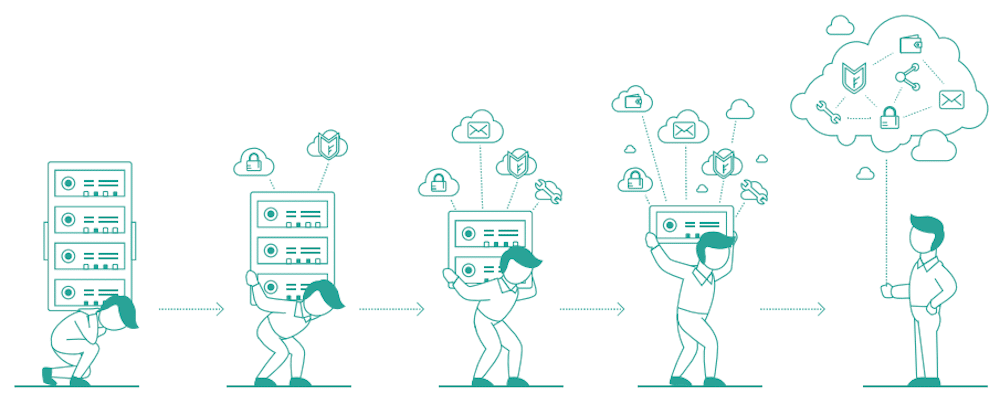
\includegraphics[width=1\textwidth]{images/jpg/cloud-evolution.png} % Ajusta el tamaño seg{\'u}n necesites
                \caption{Evoluci{\'o}n de computaci{\'o}n en la nube}
                \label{fig:CloudEvolution}
            \end{figure}            
            Las principales etapas de evoluci{\'o}n de la computaci{\'o}n en la nube, se podr{\'i}an describir las siguientes:
            
            \begin{itemize}
                \item D{\'e}cada de 1960: John MacCarthy introdujo el concepto de "time-sharing" en computadoras mainframe, donde m{\'u}ltiples usuarios pod{\'i}an utilizar un mismo sistema simult{\'a}neamente.
                \item D{\'e}cada de 1990: Se desarrollaron las primeras infraestructuras de virtualizaci{\'o}n, permitiendo ejecutar m{\'u}ltiples sistemas operativos en un mismo servidor.
                \item D{\'e}cada de 2000: Empresas como Amazon Web Services (AWS) comenzaron a ofrecer servicios de infraestructura en la nube, estableciendo un nuevo modelo de prestaci{\'o}n de servicios inform{\'a}ticos.
                \item Actualidad: La computaci{\'o}n en la nube se ha consolidado como una de las tecnolog{\'i}as fundamentales para el almacenamiento y procesamiento de datos en m{\'u}ltiples sectores.
            \end{itemize}

        \subsection{Evoluci{\'o}n del modelo virtual de Nube}
            La computaci{\'o}n en la nube se ha diseñado con el objetivo de optimizar la gesti{\'o}n de recursos tecnol{\'o}gicos, mejorando la calidad de los servicios mediante la aplicaci{\'o}n de est{\'a}ndares exigentes de la industria. Generalmente, estos servicios se alojan en centros de datos especialmente diseñados para proporcionar soluciones alineadas con buenas pr{\'a}cticas y recomendaciones de normas internacionales, como las establecidas por organismos como ISO, TIA, BICSI e ICREA, entre otros.

            El desarrollo de una infraestructura de computaci{\'o}n en la nube sigue un proceso evolutivo que busca garantizar alta disponibilidad, escalabilidad y eficiencia en el procesamiento de datos masivos. Desde la construcci{\'o}n de un centro de datos hasta la adopci{\'o}n de arquitecturas distribuidas, este proceso ha permitido a las organizaciones gestionar grandes vol{\'u}menes de informaci{\'o}n y aplicar modelos avanzados de an{\'a}lisis, aprendizaje autom{\'a}tico e IA.

            A continuaci{\'o}n, se presentan las principales etapas de esta evoluci{\'o}n (ver la Figura \ref{fig:VirtualCloudEvolution}), con un enfoque en el soporte a proyectos de ciencia de datos y an{\'a}lisis de grandes vol{\'u}menes de informaci{\'o}n.
            
            \begin{figure}[h] % La opci{\'o}n [H] obliga a poner la imagen aqu{\'i}, sin moverla
                \centering
                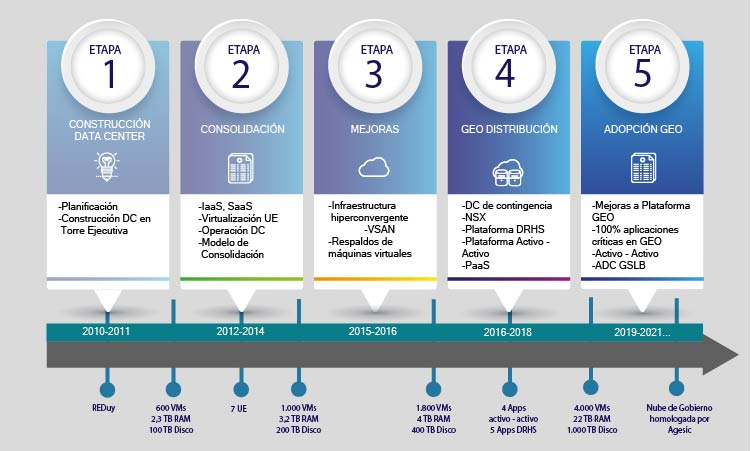
\includegraphics[width=1\textwidth]{images/jpg/Evolution_Cloud_1.jpg} % Ajusta el tamaño seg{\'u}n necesites
                \caption{Evoluci{\'o}n del modelo virtual en la nube}
                \label{fig:VirtualCloudEvolution}
            \end{figure} 
            
            Este enfoque permite alcanzar altos niveles de seguridad, disponibilidad y confiabilidad, cumpliendo con los requisitos t{\'e}cnicos en {\'a}reas clave como el suministro el{\'e}ctrico, los sistemas de climatizaci{\'o}n, la seguridad f{\'i}sica, la infraestructura civil y las comunicaciones.

            \subsubsection{Etapa 1: Construcci{\'o}n del Centro de Datos (2010 - 2011)}
                El primer paso en la evoluci{\'o}n de una infraestructura de computaci{\'o}n en la nube para ciencia de datos es la creaci{\'o}n de un centro de datos que garantice capacidad de procesamiento y almacenamiento escalable. En esta fase, se diseñan e implementan infraestructuras f{\'i}sicas capaces de soportar altas cargas de trabajo computacional, almacenamiento redundante y sistemas de comunicaci{\'o}n de alta velocidad.
            
                Se establecen bases de datos relacionales y no relacionales para manejar distintos tipos de informaci{\'o}n, desde datos estructurados hasta informaci{\'o}n semiestructurada y no estructurada. Adem{\'a}s, se consideran aspectos como la integraci{\'o}n con sensores IoT para la recolecci{\'o}n de datos en tiempo real y el aseguramiento de la continuidad operativa con sistemas de respaldo y redundancia.
            
                Esta infraestructura inicial es clave para soportar proyectos de almacenamiento de datos masivos (Big Data) y facilitar el acceso a herramientas de an{\'a}lisis en la nube.
            
            \subsubsection{Etapa 2: Consolidaci{\'o}n y Virtualizaci{\'o}n (2012 - 2014)}
                Una vez establecido el centro de datos, el siguiente paso es la optimizaci{\'o}n del uso de los recursos computacionales mediante t{\'e}cnicas de consolidaci{\'o}n y virtualizaci{\'o}n. Se implementan modelos de servicio como Infraestructura como Servicio (IaaS) y Software como Servicio (SaaS), que permiten a los investigadores y cient{\'i}ficos de datos acceder a entornos flexibles para sus proyectos sin depender de hardware f{\'i}sico propio.
            
                En esta etapa se popularizan plataformas de procesamiento distribuido como Apache Hadoop y Apache Spark, que facilitan el an{\'a}lisis de datos en cl{\'u}steres de servidores virtualizados. Adem{\'a}s, se integran herramientas de virtualizaci{\'o}n de entornos de desarrollo para que los cient{\'i}ficos de datos puedan realizar pruebas y despliegues de modelos de machine learning sin preocuparse por la gesti{\'o}n de infraestructura.
            
                El enfoque de consolidaci{\'o}n permite un uso m{\'a}s eficiente de los recursos, evitando la subutilizaci{\'o}n de servidores y optimizando el almacenamiento de datos en estructuras distribuidas y escalables.
            
            \subsubsection{Etapa 3: Incorporaci{\'o}n de Mejoras Tecnol{\'o}gicas y Computaci{\'o}n Hiperconvergente (2015 - 2016)}
                A medida que la demanda de procesamiento de datos masivos y aprendizaje autom{\'a}tico crece, se requiere una infraestructura m{\'a}s eficiente y optimizada. Se implementan arquitecturas de computaci{\'o}n hiperconvergente, integrando en un solo sistema los recursos de c{\'o}mputo, almacenamiento y redes.
            
                En esta fase, se ampl{\'i}a el uso de almacenamiento definido por software (Software Defined Storage, SDS), lo que permite gestionar grandes vol{\'u}menes de datos de manera flexible y sin depender de hardware f{\'i}sico propietario. Se incorporan soluciones como VSAN y almacenamiento distribuido, lo que facilita la gesti{\'o}n de conjuntos de datos cada vez m{\'a}s grandes y heterog{\'e}neos.
            
                Adem{\'a}s, se optimizan los sistemas de respaldo y recuperaci{\'o}n de datos para garantizar la seguridad de la informaci{\'o}n utilizada en experimentos y modelos de an{\'a}lisis predictivo. Tambi{\'e}n comienzan a adoptarse modelos de GPU Computing, lo que acelera significativamente los c{\'a}lculos en proyectos de deep learning.
            
            \subsubsection{Etapa 4: Distribuci{\'o}n Geogr{\'a}fica y Procesamiento en Tiempo Real (2016 - 2018)}
                Con el crecimiento de la ciencia de datos y el auge del Internet de las Cosas (IoT), la infraestructura de computaci{\'o}n en la nube evoluciona hacia un modelo distribuido geogr{\'a}ficamente, lo que permite reducir la latencia en el procesamiento de datos y mejorar la respuesta en tiempo real.
            
                Se crean centros de datos de contingencia y se implementan esquemas de procesamiento perimetral (Edge Computing) para acercar el an{\'a}lisis a la fuente de generaci{\'o}n de datos. Esto es crucial en aplicaciones como an{\'a}lisis de video en tiempo real, predicci{\'o}n de eventos clim{\'a}ticos y detecci{\'o}n de anomal{\'i}as en sistemas financieros.
            
                Adem{\'a}s, se implementan modelos de Plataforma como Servicio (PaaS) para facilitar el despliegue de modelos de IA en entornos productivos. Tecnolog{\'i}as como Apache Kafka y Google BigQuery comienzan a ser adoptadas para el procesamiento y an{\'a}lisis de flujos de datos en tiempo real.
            
                En esta etapa, la nube deja de ser solo un espacio de almacenamiento y se convierte en un ecosistema de procesamiento activo para proyectos de ciencia de datos, donde la velocidad de acceso a la informaci{\'o}n es cr{\'i}tica.
            
            \subsubsection{Etapa 5: Adopci{\'o}n de una Infraestructura Global e Inteligente (2019 - 2021)}
                La {\'u}ltima etapa en la evoluci{\'o}n de la computaci{\'o}n en la nube para ciencia de datos es la integraci{\'o}n de una infraestructura global, inteligente y autosuficiente. Se adopta un modelo de arquitectura distribuida, en el que los datos y los servicios se encuentran replicados en m{\'u}ltiples ubicaciones para garantizar alta disponibilidad y recuperaci{\'o}n ante desastres.
            
                Los sistemas comienzan a operar en entornos multicloud para aprovechar la diversidad de servicios ofrecidos por diferentes proveedores, optimizando costos y rendimiento. Se implementan balanceadores de carga avanzados como ADC GSLB (Global Server Load Balancing) para gestionar el tr{\'a}fico de datos y garantizar accesibilidad desde cualquier parte del mundo.
            
                Adem{\'a}s, se adopta el uso de IA para la optimizaci{\'o}n de recursos dentro de la nube, lo que permite asignar din{\'a}micamente capacidad de c{\'o}mputo y almacenamiento seg{\'u}n la demanda. Tecnolog{\'i}as como MLOps (Machine Learning Operations) facilitan la automatizaci{\'o}n del ciclo de vida de los modelos de IA, reduciendo los tiempos de implementaci{\'o}n y mejorando la eficiencia operativa.
            
                En esta fase, la nube se consolida como un pilar fundamental para el desarrollo de proyectos de Big Data, IA y an{\'a}lisis predictivo, permitiendo a las organizaciones y cient{\'i}ficos de datos escalar sus experimentos a nivel global con m{\'a}xima eficiencia.
            
        \subsection[Caracter{\'i}sticas NIST para la Clou Computing]{Caracter{\'i}sticas de la computaci{\'o}n en la nube seg{\'u}n el modelo del NIST}
            El Instituto Nacional de Est{\'a}ndares y Tecnolog{\'i}a (NIST) define la computaci{\'o}n en la nube como un modelo que permite el acceso conveniente y bajo demanda a recursos inform{\'a}ticos compartidos, con caracter{\'i}sticas espec{\'i}ficas que lo diferencian de otros modelos de prestaci{\'o}n de servicios.

            Las caracter{\'i}sticas de computaci{\'o}n en la nube seg{\'u}n el NIST son:

            \begin{figure}[h] % La opci{\'o}n [H] obliga a poner la imagen aqu{\'i}, sin moverla
                \centering
                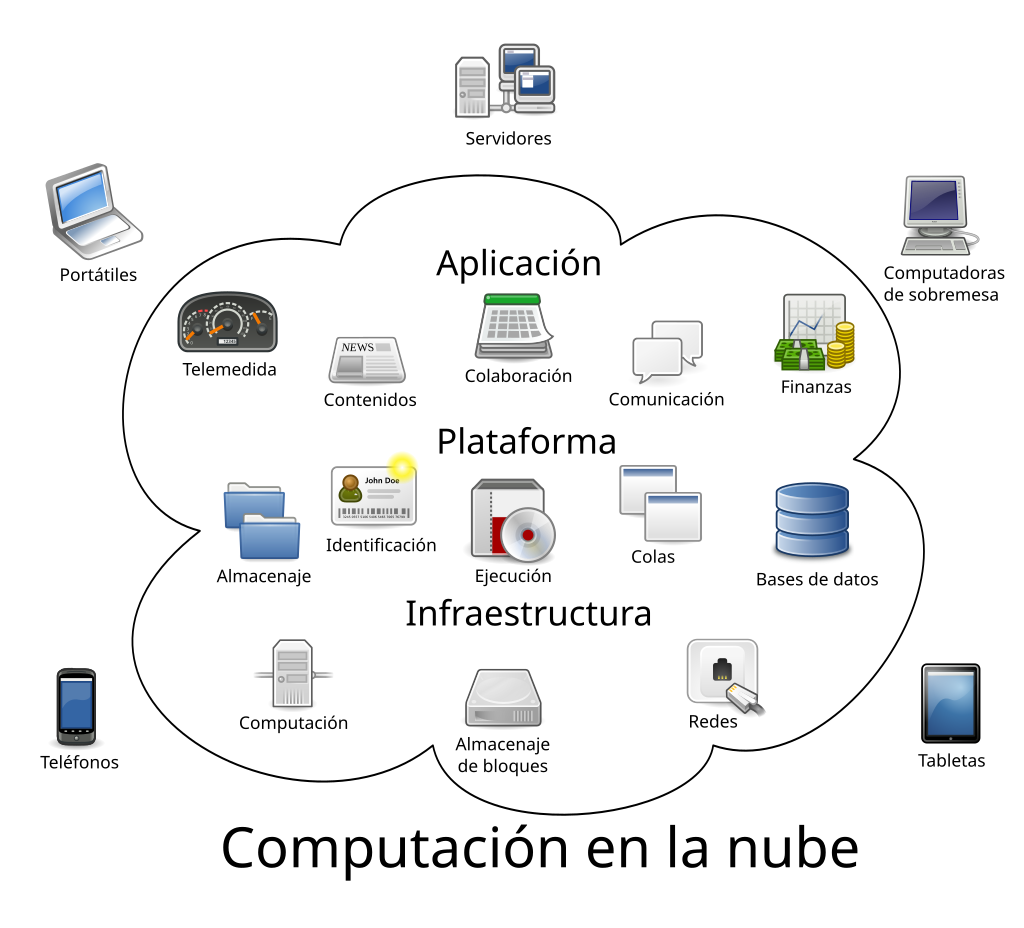
\includegraphics[width=1\textwidth]{images/svg/Cloud_computing-es.svg} % Ajusta el tamaño seg{\'u}n necesites
                \caption{Caracter{\'i}sticas de Computaci{\'o}n en la Nube seg{\'u}n NIST.}
                \label{fig:CaracteristicasCloud}
            \end{figure}
            
            \begin{itemize}
                \item Autoservicio Bajo Demanda: Los usuarios pueden obtener recursos de manera autom{\'a}tica sin intervenci{\'o}n humana.
                \item Amplio Acceso a la Red: Se accede a los servicios desde m{\'u}ltiples dispositivos sin restricciones de ubicaci{\'o}n.
                \item Pool de Recursos: Los recursos se asignan de forma din{\'a}mica entre m{\'u}ltiples clientes.
                \item Escalabilidad R{\'a}pida: La infraestructura puede adaptarse a las necesidades de los usuarios en cualquier momento.
                \item Servicio Medido: Se realiza un monitoreo del uso de los recursos para facturar en funci{\'o}n del consumo real.
            \end{itemize}
        
    \section[Modelos de despliegue]{Modelos de despliegue en la computaci{\'o}n en la nube}
        Los modelos de despliegue en la nube determinan c{\'o}mo se implementan y gestionan los servicios en funci{\'o}n de las necesidades de cada organizaci{\'o}n.
        
        Entre los modelos de Despliegue se pueden mencionar:
            
        \begin{itemize}
            \item Nube P{\'u}blica: Infraestructura compartida accesible por m{\'u}ltiples clientes.
            \item Nube Privada: Infraestructura exclusiva para una sola organizaci{\'o}n.
            \item Nube H{\'i}brida: Combinaci{\'o}n de nube p{\'u}blica y privada, optimizando recursos y seguridad.
            \item Multicloud: Uso de m{\'u}ltiples proveedores de nube para distribuir servicios y mejorar la redundancia.
        \end{itemize}
        
        \subsection[Modelos de servicios]{Modelos de servicio en la computaci{\'o}n en la nube}
            Existen diferentes modelos de servicio en la computaci{\'o}n en la nube que determinan la forma en que los recursos son ofrecidos a los usuarios.
            
            Los modelos de servicios que se ofrecen en la nube:

            \begin{itemize}
                \item SaaS: Permite acceder a aplicaciones alojadas en la nube sin necesidad de instalaci{\'o}n local. Ejemplo: Google Drive.
                \item PaaS: Ofrece un entorno de desarrollo completo para que los programadores creen aplicaciones sin gestionar la infraestructura subyacente. Ejemplo: Google App Engine.
                \item IaaS: Proporciona recursos de computaci{\'o}n como servidores, almacenamiento y redes, permitiendo a las empresas construir sus propias soluciones tecnol{\'o}gicas. Ejemplo: Amazon Web Services.
            \end{itemize}
            
        \subsection[Impacto en el {\'a}mbito empresarial]{Impacto de la computaci{\'o}n en la nube en el {\'a}mbito empresarial}
            Las empresas han encontrado en la computaci{\'o}n en la nube una soluci{\'o}n para optimizar sus operaciones, reducir costos y mejorar la eficiencia en la gesti{\'o}n de recursos tecnol{\'o}gicos.
            
            \paragraph{Beneficios en el entorno empresarial}
            \begin{itemize}
                \item Reducci{\'o}n de Costos Operativos: No se requiere comprar ni mantener servidores f{\'i}sicos, lo que disminuye los gastos en infraestructura. 
                \item Mayor Flexibilidad: Permite a las empresas adaptar su capacidad inform{\'a}tica en funci{\'o}n de la demanda sin necesidad de inversiones adicionales.
                \item Acceso Global: Los empleados pueden trabajar desde cualquier lugar, accediendo a los sistemas empresariales sin restricciones geogr{\'a}ficas.
                \item Optimizaci{\'o}n del Trabajo en Equipo: La colaboraci{\'o}n entre equipos se mejora con herramientas alojadas en la nube, permitiendo la edici{\'o}n de documentos y el acceso a informaci{\'o}n en tiempo real.
            \end{itemize}
        \subsection[Impacto en el {\'a}mbito tecnol{\'o}gico]{Impacto de la computaci{\'o}n en la nube en el {\'a}mbito tecnol{\'o}gico}
            La computaci{\'o}n en la nube ha transformado el sector tecnol{\'o}gico, facilitando el desarrollo de aplicaciones innovadoras y mejorando la eficiencia en la gesti{\'o}n de datos.
            
            \paragraph{Principales transformaciones}
            \begin{itemize}
                \item Avance de la IA y el Big Data: La nube proporciona la capacidad de procesamiento necesaria para entrenar modelos de IA y analizar grandes vol{\'u}menes de datos.
                \item Automatizaci{\'o}n de Procesos: Permite la implementaci{\'o}n de herramientas de automatizaci{\'o}n que agilizan tareas repetitivas y mejoran la productividad.
                \item Expansi{\'o}n de los Servicios en L{\'i}nea: Empresas de entretenimiento, educaci{\'o}n y comercio electr{\'o}nico han adoptado soluciones en la nube para mejorar la experiencia del usuario.
            \end{itemize}
        \subsection[Impacto en el {\'a}mbito financiero]{Impacto de la computaci{\'o}n en la nube en el {\'a}mbito financiero}
            En el sector financiero, la computaci{\'o}n en la nube ha permitido a bancos y entidades financieras no solo modernizar sus sistemas sino tambi{\'e}n mejorar la seguridad y la eficiencia de sus operaciones. La capacidad de procesar grandes vol{\'u}menes de transacciones de manera r{\'a}pida y segura sin la necesidad de infraestructuras f{\'i}sicas pesadas ha sido un cambio transformador.

            \begin{itemize}
                \item An{\'a}lisis de datos a gran escala: La nube facilita a las instituciones financieras el an{\'a}lisis de enormes conjuntos de datos para detectar tendencias de mercado, realizar evaluaciones de riesgo crediticio y detectar actividades fraudulentas. El uso de herramientas de big data en la nube permite realizar estas tareas con una precisi{\'o}n y velocidad que los sistemas tradicionales no podr{\'i}an igualar.
                \item Servicios de banca en l{\'i}nea: La adopci{\'o}n de la nube ha permitido a las entidades financieras ofrecer a sus clientes servicios de banca en l{\'i}nea m{\'a}s robustos, accesibles y seguros. Estos servicios incluyen transacciones financieras, consultas de saldo, pagos de servicios y m{\'a}s, disponibles 24/7 desde cualquier dispositivo con acceso a internet.
            \end{itemize}
        \subsection[Impacto en el sector de la salud]{Impacto de la computaci{\'o}n en la nube en el sector de la salud}
            El sector salud ha integrado la computaci{\'o}n en la nube para mejorar la gesti{\'o}n de los registros m{\'e}dicos, facilitar servicios de telemedicina y apoyar la investigaci{\'o}n m{\'e}dica. Estas aplicaciones han mejorado notablemente la eficiencia operativa y la capacidad de respuesta ante emergencias m{\'e}dicas.

            \begin{itemize}
                \item Almacenamiento de registros m{\'e}dicos: Los sistemas de salud utilizan la nube para almacenar y gestionar de forma segura los registros m{\'e}dicos electr{\'o}nicos, permitiendo a los profesionales de la salud acceder y compartir informaci{\'o}n vital del paciente de manera r{\'a}pida y segura, mejorando as{\'i} la calidad del cuidado m{\'e}dico.
                \item Telemedicina: La nube ha sido fundamental para el despliegue de servicios de telemedicina, que permiten consultas m{\'e}dicas a distancia, diagn{\'o}sticos y seguimiento de pacientes en tiempo real, facilitando el acceso a servicios m{\'e}dicos a poblaciones en {\'a}reas remotas o con movilidad reducida.
            \end{itemize}
        \subsection[Impacto en la educaci{\'o}n]{Impacto de la computaci{\'o}n en la nube en el {\'a}mbito de la educaci{\'o}n}
            Las instituciones educativas han adoptado la computaci{\'o}n en la nube para transformar la enseñanza y el aprendizaje, proporcionando herramientas que apoyan la educaci{\'o}n a distancia, el almacenamiento de contenido educativo y la gesti{\'o}n de datos estudiantiles de manera segura y escalable.
            
            \begin{itemize}
                \item Entornos de aprendizaje virtual: La nube ha permitido la creaci{\'o}n y expansi{\'o}n de plataformas de aprendizaje virtual que soportan videoconferencias, recursos educativos interactivos y herramientas de colaboraci{\'o}n que estudiantes y profesores pueden utilizar para interactuar en tiempo real, independientemente de su ubicaci{\'o}n f{\'i}sica.
                \item Gesti{\'o}n de datos estudiantiles: Las soluciones en la nube ofrecen a las escuelas y universidades la capacidad de almacenar y gestionar de manera eficiente y segura los registros acad{\'e}micos, la asistencia, las calificaciones y otros datos importantes de los estudiantes, facilitando el acceso a la informaci{\'o}n por parte de administrativos y docentes.
            \end{itemize}
        \subsection[Impacto en el sector gubernamental]{Impacto de la computaci{\'o}n en la nube en el sector gubernamental}
            Las agencias gubernamentales han implementado soluciones en la nube para mejorar la entrega de servicios p{\'u}blicos y aumentar la eficiencia operativa. La adopci{\'o}n de la nube ha permitido una mejor colaboraci{\'o}n entre diferentes entidades gubernamentales y ha facilitado el acceso p{\'u}blico a la informaci{\'o}n.

            \begin{itemize}
                \item Mejora en la prestaci{\'o}n de servicios p{\'u}blicos: La computaci{\'o}n en la nube permite a las entidades gubernamentales ofrecer servicios en l{\'i}nea m{\'a}s efectivos, como la tramitaci{\'o}n de documentos, pagos de servicios y consultas, lo que resulta en una mayor satisfacci{\'o}n ciudadana y una reducci{\'o}n en los tiempos de espera y procesamiento.
                \item Transparencia y acceso a la informaci{\'o}n: La nube facilita a las agencias del gobierno almacenar y compartir informaci{\'o}n de manera segura y accesible, promoviendo la transparencia y permitiendo a los ciudadanos acceder a datos y estad{\'i}sticas gubernamentales de manera f{\'a}cil y r{\'a}pida.
            \end{itemize}        
        \subsection[Cloud Computing e IA]{Impacto de la computaci{\'o}n en la nube y la Inteligencia Artificial}
            La integraci{\'o}n de la Inteligencia Artificial (IA) en plataformas de computaci{\'o}n en la nube ha facilitado a empresas de todos los tamaños la implementaci{\'o}n de soluciones inteligentes sin la necesidad de inversiones significativas en infraestructura propia.

            \begin{figure}[h] % La opci{\'o}n [H] obliga a poner la imagen aqu{\'i}, sin moverla
                \centering
                
\includegraphics[width=1\textwidth]{images/jpg/AICloudComputing.jpeg} % Ajusta el tamaño seg{\'u}n necesites
                \caption{IA en la nube}
                \label{fig:IA-Cloud}
            \end{figure}
            
            La IA aprovecha la capacidad de procesamiento y el almacenamiento de la nube para ofrecer servicios que van desde el an{\'a}lisis predictivo hasta el procesamiento del lenguaje natural y la automatizaci{\'o}n de tareas.

            \begin{itemize}
                \item An{\'a}lisis predictivo: Utilizando modelos estad{\'i}sticos y algoritmos de machine learning, el an{\'a}lisis predictivo en la nube ayuda a las empresas a anticipar eventos futuros bas{\'a}ndose en datos hist{\'o}ricos. Esta capacidad es utilizada en industrias como las financieras para evaluar riesgos de cr{\'e}dito y en el comercio electr{\'o}nico para personalizar recomendaciones de productos a los usuarios.
                \item Automatizaci{\'o}n de procesos: Las herramientas de IA en la nube permiten la automatizaci{\'o}n de procesos repetitivos, liberando a los empleados para que se enfoquen en tareas m{\'a}s estrat{\'e}gicas. Estas soluciones pueden mejorar significativamente la eficiencia operativa y reducir errores.
            \end{itemize}
        \subsection[Cloud Computing y Big Data]{Impacto de la computaci{\'o}n en la nube en big data}
            El manejo de grandes vol{\'u}menes de datos, o Big Data, se ha optimizado gracias a la capacidad y flexibilidad que ofrecen las soluciones de computaci{\'o}n en la nube. La nube proporciona el entorno ideal para almacenar, procesar y analizar grandes conjuntos de datos, facilitando a las organizaciones la obtenci{\'o}n de informaci{\'o}n que respalda la toma de decisiones estrat{\'e}gicas.

            \begin{itemize}
                \item Almacenamiento y gesti{\'o}n de datos: La nube ofrece opciones escalables y seguras para el almacenamiento de grandes cantidades de datos, asegurando la disponibilidad y la integridad de la informaci{\'o}n. Las empresas pueden gestionar sus datos de manera m{\'a}s eficiente, adaptando los recursos a la demanda.
                \item An{\'a}lisis de datos: Con herramientas de an{\'a}lisis integradas, la nube permite a las empresas explorar complejos conjuntos de datos para identificar tendencias, realizar an{\'a}lisis sectoriales, y desarrollar nuevos productos o servicios basados en conocimiento obtenidos a partir del an{\'a}lisis de datos.
            \end{itemize}
        \subsection[Cloud Computing e IoT]{Impacto de la computaci{\'o}n en la nube en internet de las cosas (IoT)}
            El Internet de las Cosas se ha expandido enormemente con la ayuda de la computaci{\'o}n en la nube. Los dispositivos IoT generan grandes cantidades de datos que necesitan ser procesados y analizados en tiempo real. La nube ofrece una plataforma robusta y escalable para conectar y gestionar estos dispositivos, facilitando la integraci{\'o}n y sincronizaci{\'o}n de datos en una red global.

            \begin{figure}[h] % La opci{\'o}n [H] obliga a poner la imagen aqu{\'i}, sin moverla
                \centering
                
\includegraphics[width=1\textwidth]{images/jpg/IA-IoT.jpg} % Ajusta el tamaño seg{\'u}n necesites
                \caption{IoT y la Nube}
                \label{fig:IoT-Cloud}
            \end{figure}
            
            \begin{itemize}
                \item Gesti{\'o}n de Dispositivos IoT: La nube permite la gesti{\'o}n centralizada de dispositivos IoT, desde sensores en una planta industrial hasta dispositivos portatiles de consumo. Esto incluye la actualizaci{\'o}n de software, la monitorizaci{\'o}n del estado de los dispositivos y la respuesta a incidentes en tiempo real.
                \item An{\'a}lisis en Tiempo Real: Utilizando la capacidad de procesamiento en la nube, los datos recogidos por dispositivos IoT pueden ser analizados casi instant{\'a}neamente para detectar anomal{\'i}as, optimizar procesos y mejorar la toma de decisiones basada en datos actuales.
            \end{itemize}
            
        \subsection[Cloud Computing y Blockchain]{Impacto de la computaci{\'o}n en la nube al blockchain}
            La tecnolog{\'i}a Blockchain se ha visto potenciada por su implementaci{\'o}n en la nube, permitiendo a las empresas y desarrolladores crear y gestionar redes blockchain sin la necesidad de desarrollar su propia infraestructura. La computaci{\'o}n en la nube proporciona la seguridad, escalabilidad y eficiencia necesarias para operar blockchain, lo cual es vital para transacciones y contratos inteligentes.

            \begin{itemize}
                \item Desarrollo de Aplicaciones Blockchain: La nube ofrece plataformas especializadas que simplifican el desarrollo de aplicaciones blockchain, proporcionando herramientas preconfiguradas y servicios gestionados que aceleran el despliegue y la adopci{\'o}n de esta tecnolog{\'i}a.
                \item Seguridad y Escalabilidad: Al operar en la nube, las soluciones blockchain se benefician de la infraestructura de seguridad avanzada y la capacidad de escalar recursos r{\'a}pidamente seg{\'u}n las necesidades del sistema.
            \end{itemize}
        \subsection{Seguridad en la computaci{\'o}n en la nube}
            La seguridad es una de las {\'a}reas m{\'a}s atendidas dentro de la computaci{\'o}n en la nube. Los proveedores invierten en protocolos avanzados para proteger los datos de sus clientes contra accesos no autorizados, p{\'e}rdidas o robos. Este esfuerzo incluye la implementaci{\'o}n de firewalls, cifrado de datos, y sistemas de autenticaci{\'o}n y autorizaci{\'o}n para controlar el acceso a la informaci{\'o}n.

            \begin{itemize}
                \item Cifrado de Datos: El cifrado transforma la informaci{\'o}n clara en un c{\'o}digo ilegible sin la clave adecuada. Este proceso es vital para proteger los datos durante su transmisi{\'o}n y mientras est{\'a}n almacenados en los servidores de la nube.
                \item Gesti{\'o}n de Identidades y Accesos: La gesti{\'o}n de identidades asegura que solo los usuarios autorizados puedan acceder a aplicaciones y datos espec{\'i}ficos. Los sistemas de gesti{\'o}n de accesos en la nube permiten a las organizaciones controlar c{\'o}mo los usuarios interact{\'u}an con los recursos en la nube.
            \end{itemize}
        \subsection{Realidad aumentada y realidad virtual en la nube}
            La computaci{\'o}n en la nube est{\'a} jugando un papel transformador en el desarrollo y despliegue de aplicaciones de realidad aumentada (RA) y realidad virtual (RV). Al proporcionar potencia de procesamiento y almacenamiento, la nube permite que estas tecnolog{\'i}as sean m{\'a}s accesibles y asequibles, facilitando experiencias inmersivas en diversos sectores como la educaci{\'o}n, el entretenimiento y el diseño industrial.
            
            Desarrollo y hospedaje de aplicaciones: Las plataformas en la nube ofrecen el entorno necesario para desarrollar y alojar aplicaciones de RA y RV, reduciendo los costos de entrada y permitiendo a los creadores enfocarse en innovar en el contenido sin preocuparse por la capacidad de procesamiento o el almacenamiento

        \subsection{Implementaci{\'o}n y uso de RA y RV}
            En el sector educativo, la RA y la RV ofrecen m{\'e}todos nuevos y atractivos para enseñar conceptos complejos a trav{\'e}s de simulaciones y entornos inmersivos. Herramientas como Google Expeditions permiten realizar viajes virtuales a lugares hist{\'o}ricos o realizar exploraciones cient{\'i}ficas, mejorando el aprendizaje experiencial. Por su parte, aplicaciones como CoSpaces Edu posibilitan que los estudiantes diseñen sus propios mundos de RA y RV, fomentando la creatividad y el pensamiento computacional.
            
            En el {\'a}mbito de la salud, la implementaci{\'o}n de la RA y la RV ha permitido avances significativos en la formaci{\'o}n m{\'e}dica y la rehabilitaci{\'o}n. Plataformas como Touch Surgery ofrecen simulaciones quir{\'u}rgicas en RV para que los profesionales de la salud puedan practicar procedimientos complejos en un entorno seguro y controlado. Adem{\'a}s, tecnolog{\'i}as como Microsoft HoloLens se utilizan en cirug{\'i}a asistida por RA, proporcionando visualizaci{\'o}n en tiempo real de datos m{\'e}dicos y mejorando la precisi{\'o}n durante las intervenciones.
            
            En el diseño industrial y la manufactura, las soluciones de RA y RV est{\'a}n revolucionando la manera en que los productos son conceptualizados y desarrollados. Programas como Autodesk VRED permiten la visualizaci{\'o}n de modelos 3D en entornos virtuales antes de pasar a la producci{\'o}n f{\'i}sica, lo que facilita la detecci{\'o}n de errores en las fases tempranas del diseño. Asimismo, el uso de Unreal Engine y Unity, dos de las plataformas de desarrollo m{\'a}s populares, permite la creaci{\'o}n de prototipos virtuales interactivos que pueden integrarse con dispositivos como Oculus Rift o HTC Vive para realizar pruebas de funcionalidad y diseño ergon{\'o}mico.
            
            \subsection[La normativa y la nube]{Importancia del cumplimiento normativo en la nube}
            
            El cumplimiento normativo en la nube es vital para asegurar que las operaciones de las empresas est{\'e}n en conformidad con las leyes y regulaciones locales e internacionales. Esto incluye regulaciones sobre protecci{\'o}n de datos personales, como el GDPR en Europa y leyes similares en otras regiones.
            
            \begin{itemize}
                \item Gesti{\'o}n del Cumplimiento en la Nube: Las empresas deben garantizar que sus operaciones en la nube cumplan con las leyes de cada pa{\'i}s donde operan. Esto puede requerir que los datos se almacenen y procesen en regiones espec{\'i}ficas.
                \item Auditor{\'i}a y Transparencia: Las plataformas de servicios en la nube como AWS, Microsoft Azure y Google Cloud ofrecen herramientas integradas de auditor{\'i}a que permiten a las organizaciones monitorizar y registrar el acceso y uso de los datos, facilitando el cumplimiento de normas de seguridad y privacidad.
                \item Certificaciones y Est{\'a}ndares Internacionales: Es esencial que los proveedores de servicios en la nube cuenten con certificaciones como ISO/IEC 27001 para la gesti{\'o}n de la seguridad de la informaci{\'o}n y el cumplimiento de normativas espec{\'i}ficas del sector, como la HIPAA para el manejo de informaci{\'o}n m{\'e}dica en los Estados Unidos.
                \item Cifrado y Protecci{\'o}n de Datos: La implementaci{\'o}n de t{\'e}cnicas de cifrado de extremo a extremo y la gesti{\'o}n de claves criptogr{\'a}ficas se consideran pr{\'a}cticas obligatorias para proteger la integridad y la confidencialidad de los datos sensibles almacenados en la nube.
            \end{itemize}
            
            
        \subsection[Recuperaci{\'o}n ante desastres en la nube]{Continuidad del negocio y recuperaci{\'o}n ante desastres en la nube}
            La computaci{\'o}n en la nube ofrece soluciones para la continuidad del negocio y la recuperaci{\'o}n ante desastres. Estas soluciones aseguran que las operaciones comerciales puedan continuar con el m{\'i}nimo de interrupciones despu{\'e}s de incidentes adversos.
            
            Estrategias de implementaci{\'o}n:

            \begin{itemize}
                \item Replicaci{\'o}n de datos: La replicaci{\'o}n de datos entre m{\'u}ltiples zonas geogr{\'a}ficas asegura que, en caso de una falla en una zona, los datos sigan siendo accesibles desde otra ubicaci{\'o}n.
                \item Recuperaci{\'o}n automatizada: Los sistemas automatizados de recuperaci{\'o}n ayudan a restaurar aplicaciones y datos a su estado operativo habitual en cuesti{\'o}n de minutos, garantizando as{\'i} la operatividad continua.
            \end{itemize}
    \section[Cloud Computing seg{\'u}n NIST]{Caracter{\'i}sticas seg{\'u}n el modelo del NIST (acceso bajo demanda, elasticidad, recursos compartidos, etc.)}
        NIST define cinco caracter{\'i}sticas esenciales que diferencian a la computaci{\'o}n en la nube de otros modelos de prestaci{\'o}n de servicios tecnol{\'o}gicos. Estas caracter{\'i}sticas aseguran que los servicios de nube sean accesibles, flexibles y eficientes.
        
        \subsection{NIST y las caracter{\'i}sticas de Cloud Computing}
            \begin{itemize}
                \item Autoservicio bajo demanda: El autoservicio bajo demanda permite a los usuarios configurar y manejar sus recursos computacionales, como el poder de procesamiento y el almacenamiento, sin necesidad de intervenci{\'o}n directa de los proveedores de servicios. Esto habilita a las empresas a desplegar r{\'a}pidamente aplicaciones y servicios, ajustando los recursos a las necesidades fluctuantes sin esperas ni complicaciones.
                \item Amplio Acceso a la Red - Conectividad y Disponibilidad: Esta caracter{\'i}stica asegura que los servicios y recursos de la nube sean accesibles a trav{\'e}s de cualquier plataforma est{\'a}ndar, como computadoras de escritorio, laptops, y dispositivos m{\'o}viles, mediante mecanismos que requieren m{\'i}nima gesti{\'o}n o interacci{\'o}n directa con el proveedor del servicio. El acceso a la red es esencial para garantizar que los usuarios puedan conectarse a sus recursos en la nube desde cualquier lugar y en cualquier momento.
                \item Agrupaci{\'o}n de Recursos - Recursos Compartidos en la Nube:  Los sistemas de nube utilizan un modelo de agrupaci{\'o}n de recursos para servir a m{\'u}ltiples consumidores con diferentes necesidades f{\'i}sicas y virtuales, asignadas y reasignadas seg{\'u}n la demanda. Este modelo maximiza la eficiencia del uso de los recursos al permitir que diferentes clientes utilicen el mismo pool de servidores, almacenamiento o ancho de banda, gestionando de forma din{\'a}mica la asignaci{\'o}n seg{\'u}n los requerimientos de cada usuario. 
            \end{itemize}
        \subsection[Beneficios de Cloud Computing]{Beneficios de las caracter{\'i}sticas del modelo NIST}
            \begin{itemize}
                \item Las caracter{\'i}sticas definidas por el NIST optimizan la entrega de servicios en la nube al mejorar la accesibilidad, la eficiencia y la flexibilidad de los recursos tecnol{\'o}gicos. 
                \item Esto permite a las empresas ser m{\'a}s {\'a}giles, responder m{\'a}s r{\'a}pidamente a los cambios del mercado y reducir costos operativos.
            \end{itemize}
        \subsection[Desaf{\'i}os de Cloud Computing]{Desaf{\'i}os asociados con las caracter{\'i}sticas del NIST}
            \begin{itemize}
                \item A pesar de los beneficios, las caracter{\'i}sticas esenciales de la nube tambi{\'e}n presentan desaf{\'i}os, especialmente en t{\'e}rminos de seguridad y privacidad de los datos.
                \item La gesti{\'o}n de estos desaf{\'i}os requiere una atenci{\'o}n meticulosa a las pol{\'i}ticas de seguridad, las configuraciones de privacidad y el cumplimiento normativo.
            \end{itemize}
        \subsection{Modelos de servicios}
            Los modelos de servicio en la computaci{\'o}n en la nube definen las distintas maneras en que los recursos de tecnolog{\'i}a inform{\'a}tica pueden ser entregados a trav{\'e}s de Internet. Estos modelos son fundamentales para entender c{\'o}mo las empresas y los consumidores interact{\'u}an con la tecnolog{\'i}a en la nube, proporcionando flexibilidad, escalabilidad y acceso a tecnolog{\'i}as avanzadas sin grandes inversiones en hardware f{\'i}sico.
            
            \begin{figure}[h] % La opci{\'o}n [H] obliga a poner la imagen aqu{\'i}, sin moverla
                \centering
                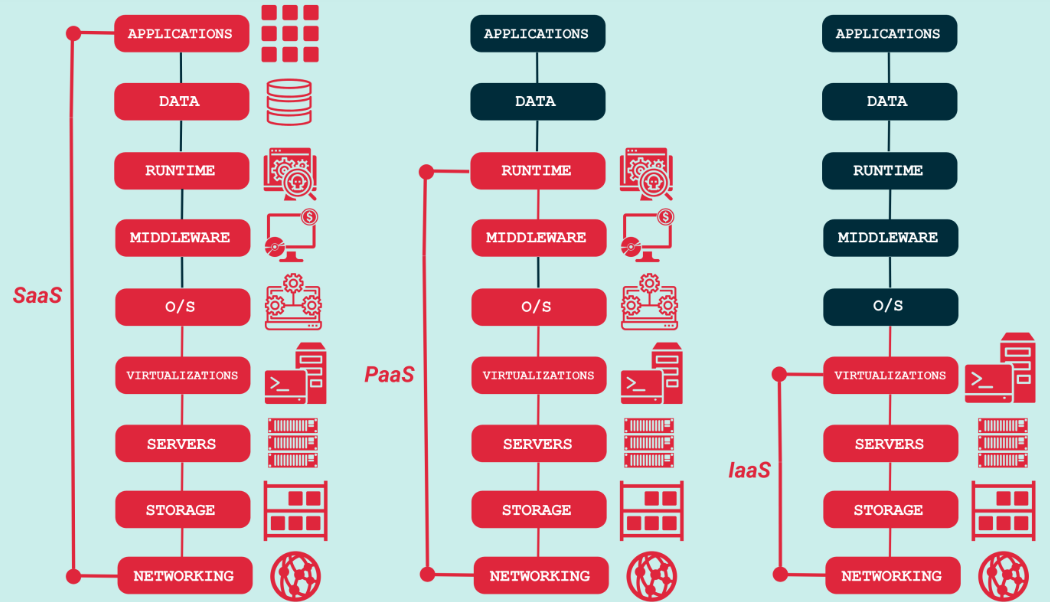
\includegraphics[width=1\textwidth]{images/png/ModelosCloudComputing.png} % Ajusta el tamaño seg{\'u}n necesites
                \caption{Evoluci{\'o}n de computaci{\'o}n en la nube}
                \label{fig:VirtualCloudEvolution}
            \end{figure}
                
            \subsubsection{Software como servicio (SaaS)}
                El modelo de Software como Servicio, o SaaS, implica el uso de aplicaciones de software a trav{\'e}s de Internet como un servicio. En lugar de instalar y mantener software, los usuarios acceden a aplicaciones a trav{\'e}s de un navegador web, gestionado por proveedores tercerizados. Las aplicaciones se alojan en servidores remotos, y los proveedores se encargan de todo el mantenimiento, incluida la actualizaci{\'o}n de software y la seguridad.

                \begin{figure}[h] % La opci{\'o}n [H] obliga a poner la imagen aqu{\'i}, sin moverla
                    \centering
                    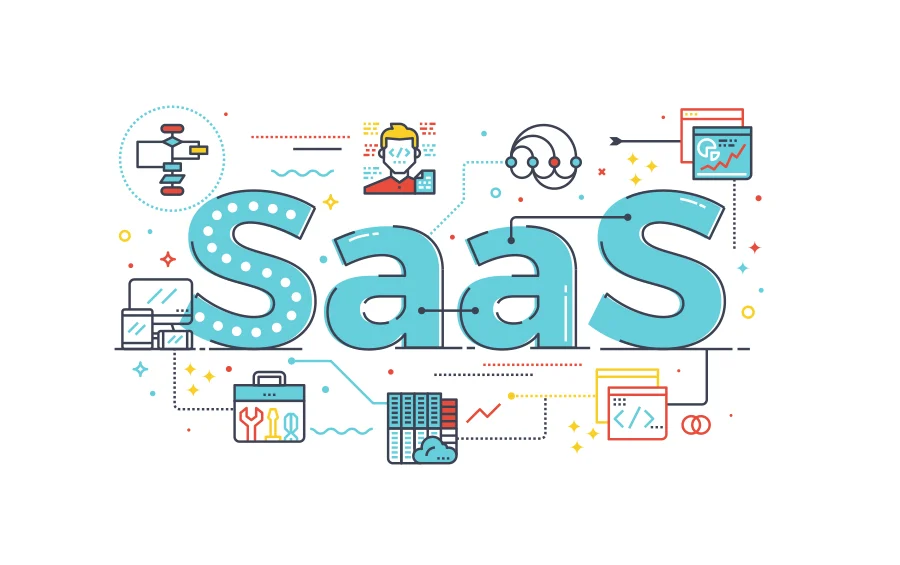
\includegraphics[width=1\textwidth]{images/png/SaaS.png} % Ajusta el tamaño seg{\'u}n necesites
                    \caption{Caracter{\'i}sticas de SaaS}
                    \label{fig:VirtualCloudEvolution}
                \end{figure}
                
                \paragraph{Ventajas del SaaS}
                    \begin{itemize}
                        \item Mantenimiento Reducido: Los usuarios no necesitan preocuparse por el mantenimiento del software ni por las actualizaciones de hardware.
                        \item Costo-Efectividad: Reduce los costos al eliminar la necesidad de software y hardware bajo licencia.
                        \item Accesibilidad: Proporciona acceso desde cualquier lugar, lo cual es ideal para empresas con empleados remotos.
                    \end{itemize}
                \paragraph{Aplicaciones Comunes de SaaS}
                    \begin{itemize}
                        \item Herramientas de productividad empresarial como Microsoft 365 y Google Workspace.
                        \item Aplicaciones de CRM como Salesforce.
                        \item Soluciones de contabilidad y facturaci{\'o}n como QuickBooks Online.
                    \end{itemize}
                \paragraph{Ventajas operacionales de SaaS}
                    \begin{itemize}
                        \item Reducci{\'o}n de la Carga de TI: SaaS elimina la necesidad de que las organizaciones instalen, actualicen y mantengan infraestructura y aplicaciones de software, delegando estas tareas a un proveedor externo. Esta externalizaci{\'o}n permite que los departamentos de TI se enfoquen en tareas m{\'a}s estrat{\'e}gicas que directamente impactan el crecimiento y la innovaci{\'o}n del negocio.
                        \item Acceso Global y Movilidad: La capacidad de acceder a aplicaciones de software desde cualquier lugar del mundo a trav{\'e}s de Internet es particularmente beneficiosa para empresas con una fuerza laboral dispersa geogr{\'a}ficamente. Esta caracter{\'i}stica asegura que todos los empleados, independientemente de su ubicaci{\'o}n, tengan acceso a herramientas necesarias para su trabajo diario, usando simplemente un navegador web.
                    \end{itemize}
                \paragraph{Desaf{\'i}os de seguridad y datos en SaaS}
                    \begin{itemize}
                        \item Gesti{\'o}n de la Seguridad de Datos: Mientras los proveedores de SaaS generalmente implementan medidas de seguridad robustas, las organizaciones deben ser diligentes en entender y evaluar estas medidas para asegurarse de que cumplen con sus propios est{\'a}ndares de seguridad y los reglamentos de la industria.
                        \item Control de Datos: A pesar de las ventajas, una preocupaci{\'o}n persistente con SaaS es el control limitado sobre los datos. Las empresas deben evaluar cuidadosamente los acuerdos de nivel de servicio (SLAs) para asegurarse de que tienen suficiente control sobre sus datos y que estos pueden ser recuperados o transferidos si cambian de proveedor de SaaS o vuelven a una soluci{\'o}n interna.
                    \end{itemize}
        \subsection[Evoluci{\'o}n de PaaS y su impacto]{Evoluci{\'o}n del PaaS y su impacto en el desarrollo de aplicaciones}
            En el {\'a}mbito de la computaci{\'o}n en la nube, el modelo PaaS (ver Figura \ref{fig:PaaSEvolution}) ha emergido como una soluci{\'o}n clave para acelerar el ciclo de vida del desarrollo de software. Este enfoque proporciona a los equipos de desarrollo un entorno integrado, que simplifica la creaci{\'o}n, prueba y despliegue de aplicaciones sin la necesidad de gestionar los recursos de infraestructura subyacentes. Al abstraer la complejidad operativa, PaaS permite a los desarrolladores concentrarse en la programaci{\'o}n y la innovaci{\'o}n de funcionalidades, apoy{\'a}ndose en herramientas y servicios que se actualizan de manera continua. Adem{\'a}s, la automatizaci{\'o}n inherente de sus procesos reduce tiempos de entrega y mejora la eficiencia en la implementaci{\'o}n de nuevas soluciones digitales.
            
            \begin{figure}[h] % La opci{\'o}n [H] obliga a poner la imagen aqu{\'i}, sin moverla
                \centering
                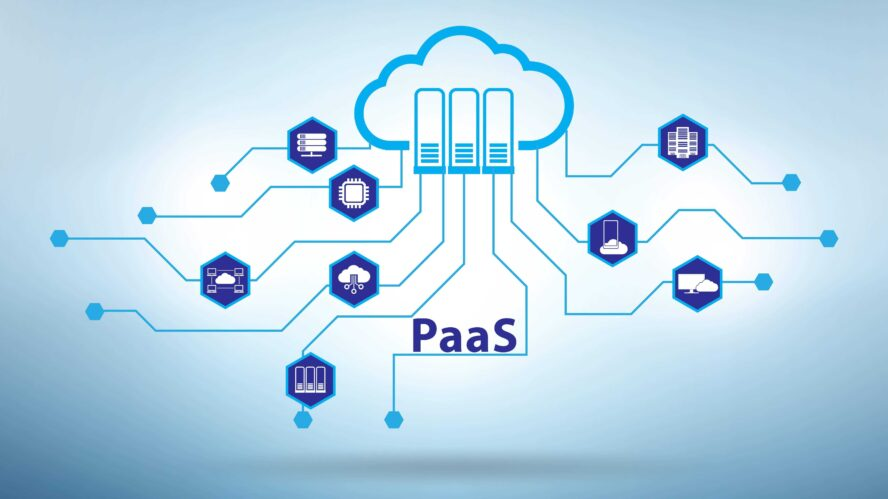
\includegraphics[width=1\textwidth]{images/jpg/PaaS.jpg} % Ajusta el tamaño seg{\'u}n necesites
                \caption{Caracter{\'i}sticas de PaaS}
                \label{fig:PaaSEvolution}
            \end{figure}
            
            \begin{itemize}
                \item Innovaci{\'o}n en Desarrollo de Software: PaaS ofrece un conjunto de herramientas de desarrollo de software que se actualizan constantemente con las {\'u}ltimas tecnolog{\'i}as, permitiendo a los desarrolladores innovar y experimentar sin la preocupaci{\'o}n de mantener el entorno de desarrollo.
                \item Automatizaci{\'o}n del Despliegue: PaaS proporciona capacidades de automatizaci{\'o}n para el despliegue de aplicaciones, lo que reduce significativamente el tiempo y el esfuerzo necesarios para lanzar nuevas aplicaciones o actualizar las existentes. Esta automatizaci{\'o}n ayuda a garantizar que las aplicaciones puedan ser desarrolladas, probadas y lanzadas de manera m{\'a}s r{\'a}pida y con menos errores.
            \end{itemize}
            
            \subsubsection{Paas para desarrollo colaborativo}
                \begin{itemize}
                    \item Plataformas Colaborativas: PaaS no solo simplifica el desarrollo de aplicaciones, sino que tambi{\'e}n promueve un ambiente colaborativo donde equipos distribuidos pueden trabajar juntos en tiempo real, independientemente de las barreras geogr{\'a}ficas.
                    \item Herramientas Integradas: Desde control de versiones hasta herramientas de seguimiento de errores y gesti{\'o}n de proyectos, PaaS ofrece un conjunto integrado de herramientas que facilitan el ciclo de vida completo del desarrollo de software.
                \end{itemize}
            \subsubsection{Desaf{\'i}os de seguridad en PaaS}
                \begin{itemize}
                    \item Dependencia del Proveedor: A medida que las empresas se vuelven dependientes de un {\'u}nico proveedor de PaaS, surge el riesgo de bloqueo, donde cambiar a otro proveedor puede resultar dif{\'i}cil y costoso.
                    \item Seguridad Multitenant: Las plataformas PaaS a menudo implementan un modelo multitenant donde m{\'u}ltiples usuarios comparten la misma infraestructura. La gesti{\'o}n adecuada de la seguridad en estos ambientes es crucial para prevenir el acceso no autorizado entre sistemas de usuario.
                \end{itemize}
        \subsection{IaaS para escalabilidad empresarial}
            
            \begin{figure}[h] % La opci{\'o}n [H] obliga a poner la imagen aqu{\'i}, sin moverla
                \centering
                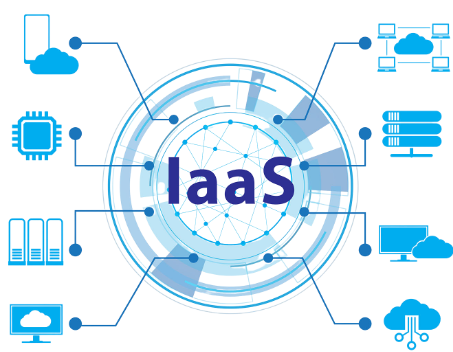
\includegraphics[width=1\textwidth]{images/png/IaaS.png} % Ajusta el tamaño seg{\'u}n necesites
                \caption{Caracter{\'i}sticas de IaaS}
                \label{fig:IaaSEvolution}
            \end{figure}
            
            \begin{itemize}
                \item Escalado Din{\'a}mico: IaaS es ideal para empresas que experimentan variaciones significativas en la demanda, proporcionando capacidad de escalar recursos r{\'a}pidamente hacia arriba o hacia abajo seg{\'u}n las necesidades del negocio.
                \item Optimizaci{\'o}n de Costos: Al utilizar IaaS, las empresas solo pagan por los recursos que usan, lo que permite una mayor flexibilidad en la gesti{\'o}n de costos operacionales y de capital.
            \end{itemize}
        \subsubsection{Retos t{\'e}cnicos y operativos en IaaS}
            \begin{itemize}
                \item Gesti{\'o}n de la Infraestructura: Aunque IaaS ofrece control sobre la infraestructura, tambi{\'e}n impone la carga de gestionar esta infraestructura, lo que puede requerir un conocimiento t{\'e}cnico significativo y recursos dedicados.
                \item Compatibilidad y Migraci{\'o}n: Migrar sistemas existentes a IaaS puede presentar desaf{\'i}os t{\'e}cnicos, especialmente en t{\'e}rminos de compatibilidad con hardware y software, y puede requerir reconfiguraci{\'o}n significativa de las aplicaciones existentes.
            \end{itemize}
    \section[Modelos de despliegue]{Modelos de despliegue: nube p{\'u}blica, privada, h{\'i}brida y multicloud}
        Los modelos de despliegue en la computaci{\'o}n en la nube se refieren a las distintas formas en que los recursos de TI se distribuyen y acceden a trav{\'e}s de diferentes arquitecturas de nube. Estos modelos se definen seg{\'u}n el grado de control, propiedad y accesibilidad que las organizaciones o individuos tienen sobre los recursos de infraestructura, almacenamiento y aplicaciones que utilizan. La elecci{\'o}n del modelo adecuado depende de factores como la sensibilidad de los datos, los requisitos regulatorios, el presupuesto disponible y los objetivos estrat{\'e}gicos de la organizaci{\'o}n.

        \begin{figure}[h] % La opci{\'o}n [H] obliga a poner la imagen aqu{\'i}, sin moverla
            \centering
            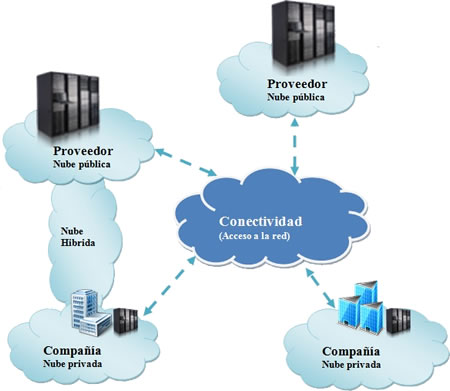
\includegraphics[width=1\textwidth]{images/jpg/tiposdenube.jpg} % Ajusta el tamaño seg{\'u}n necesites
            \caption{Tipos de Cloud}
            \label{fig:CloudTypes}
        \end{figure}
        
        Los cuatro modelos predominantes de despliegue en la nube son la nube p{\'u}blica, la nube privada, la nube h{\'i}brida y el enfoque multicloud. Cada uno ofrece un conjunto de caracter{\'i}sticas diferenciadas, que responden a necesidades espec{\'i}ficas en t{\'e}rminos de seguridad, escalabilidad, rendimiento y costo. A continuaci{\'o}n, se describen de manera detallada estos modelos, junto con sus ventajas y desaf{\'i}os asociados.
        
        \subsection{Nube p{\'u}blica}
            La nube p{\'u}blica es un modelo de prestaci{\'o}n de servicios de computaci{\'o}n que proporciona recursos compartidos a trav{\'e}s de Internet. En este modelo, los servicios son ofrecidos por proveedores especializados como Amazon Web Services (AWS), Microsoft Azure o Google Cloud Platform (GCP), quienes poseen y operan la infraestructura f{\'i}sica subyacente. El acceso a los recursos de c{\'o}mputo, almacenamiento y redes se realiza bajo demanda, permitiendo a los usuarios escalar sus operaciones de acuerdo con las necesidades espec{\'i}ficas de su negocio, sin la obligaci{\'o}n de invertir en infraestructura propia.
            
            Este enfoque se caracteriza por su apertura y disponibilidad, ya que los servicios en la nube p{\'u}blica pueden ser utilizados por cualquier organizaci{\'o}n o usuario individual mediante un esquema de pago por uso. Esto convierte a la nube p{\'u}blica en una opci{\'o}n sumamente flexible y econ{\'o}mica, ideal para organizaciones que requieren una r{\'a}pida provisi{\'o}n de recursos tecnol{\'o}gicos, sin las complejidades administrativas de mantener sus propios centros de datos.
            
            \subsubsection{Ventajas de la nube p{\'u}blica}
                Entre las principales ventajas de la nube p{\'u}blica se encuentra la optimizaci{\'o}n de costos operativos. Las organizaciones no necesitan realizar inversiones iniciales en infraestructura f{\'i}sica, ya que el modelo de pago por consumo permite adaptar los gastos al uso real de los servicios. Esta flexibilidad econ{\'o}mica es especialmente beneficiosa para pequeñas y medianas empresas que buscan maximizar sus recursos sin comprometer su capacidad tecnol{\'o}gica (Mell \& Grance, 2011).
                
                Otra ventaja destacable es la alta escalabilidad que ofrecen estos entornos. Los proveedores de nube p{\'u}blica disponen de vastos centros de datos distribuidos globalmente, lo que garantiza la disponibilidad continua de recursos y la posibilidad de gestionar picos de demanda de manera eficiente. Asimismo, la redundancia y la recuperaci{\'o}n ante desastres est{\'a}n integradas en los servicios p{\'u}blicos, mejorando la continuidad del negocio y la resiliencia frente a fallos.
                
            \subsubsection{Desaf{\'i}os de la nube p{\'u}blica}
                A pesar de sus ventajas, la nube p{\'u}blica presenta desaf{\'i}os significativos relacionados principalmente con la seguridad y el cumplimiento normativo. Al ser un entorno compartido, las organizaciones deben confiar en los mecanismos de protecci{\'o}n implementados por el proveedor, lo que puede representar un riesgo para aquellas que manejan datos sensibles o confidenciales sujetos a regulaciones estrictas como GDPR o HIPAA (Fern{\'a}ndez et al., 2014).
                
                Adicionalmente, la dependencia de servicios externos puede limitar el control directo sobre la infraestructura y las aplicaciones, dificultando la personalizaci{\'o}n profunda o la integraci{\'o}n con sistemas heredados. Este nivel de dependencia puede generar incertidumbre en t{\'e}rminos de calidad del servicio, tiempo de respuesta ante incidencias y adaptaci{\'o}n a necesidades espec{\'i}ficas del negocio.

        \subsection{Nube privada}
            La nube privada es un modelo de computaci{\'o}n en la nube que proporciona un entorno exclusivo y dedicado a una sola organizaci{\'o}n. En este escenario, la infraestructura y los servicios son utilizados de manera exclusiva, lo que permite un mayor control y personalizaci{\'o}n de los recursos tecnol{\'o}gicos. Las nubes privadas pueden ser alojadas dentro de las propias instalaciones de la organizaci{\'o}n (on-premises) o gestionadas por terceros en centros de datos externos, aunque siguen estando aisladas de otras instancias de clientes.
            
            Este modelo es especialmente adecuado para organizaciones que deben cumplir con pol{\'i}ticas rigurosas de seguridad, confidencialidad y cumplimiento normativo, como entidades gubernamentales, instituciones financieras o compañ{\'i}as del sector salud. La nube privada ofrece la posibilidad de adaptar el entorno tecnol{\'o}gico a los requerimientos espec{\'i}ficos del negocio, mejorando el rendimiento y la seguridad.
            
            \subsubsection{Ventajas de la nube privada}
                Una de las ventajas m{\'a}s destacadas de la nube privada es el control absoluto que proporciona sobre los recursos y la seguridad de la informaci{\'o}n. Las organizaciones pueden implementar pol{\'i}ticas personalizadas de acceso, cifrado y auditor{\'i}a, garantizando el cumplimiento de normativas internas y externas. Esto es fundamental para sectores que manejan datos cr{\'i}ticos, como el financiero o el sanitario (Zhang et al., 2010).
                
                Adem{\'a}s, la personalizaci{\'o}n de la infraestructura permite optimizar el rendimiento de las aplicaciones y sistemas cr{\'i}ticos, adaptando los recursos a las necesidades espec{\'i}ficas de cada {\'a}rea funcional. Esta capacidad de configuraci{\'o}n detallada puede traducirse en una mayor eficiencia operativa y en una mejor experiencia de usuario final.
                
            \subsubsection{Desaf{\'i}os de la nube privada}
                El principal desaf{\'i}o de la nube privada es su elevado costo de implementaci{\'o}n y mantenimiento. La adquisici{\'o}n de hardware, la construcci{\'o}n de centros de datos, la gesti{\'o}n de la seguridad y la contrataci{\'o}n de personal especializado suponen una inversi{\'o}n considerable que no siempre es viable para todas las organizaciones (Buyya et al., 2013).
                
                Adicionalmente, la responsabilidad de asegurar la disponibilidad, la escalabilidad y la actualizaci{\'o}n tecnol{\'o}gica recae completamente en la organizaci{\'o}n propietaria. Esto puede generar limitaciones en la capacidad de adaptaci{\'o}n a nuevas tecnolog{\'i}as y en la respuesta ante incrementos inesperados de la demanda de recursos.
                
        \subsection{Nube h{\'i}brida}
            La nube h{\'i}brida es un modelo de despliegue que integra elementos de nubes p{\'u}blicas y privadas, permitiendo a las organizaciones combinar las ventajas de ambos entornos en una {\'u}nica arquitectura coherente. Este enfoque posibilita que los recursos m{\'a}s sensibles o cr{\'i}ticos se mantengan en la nube privada, mientras que las cargas de trabajo menos exigentes o temporales se deleguen a la nube p{\'u}blica, optimizando costos y recursos.
            
            El modelo h{\'i}brido ofrece una soluci{\'o}n intermedia para las organizaciones que buscan mantener el control de sus datos y aplicaciones estrat{\'e}gicas, sin renunciar a la flexibilidad y la escalabilidad que proporciona la nube p{\'u}blica. Esto permite crear entornos din{\'a}micos que pueden responder r{\'a}pidamente a las fluctuaciones en las demandas del negocio.
            
            \subsubsection{Ventajas de la nube h{\'i}brida}
                Una de las principales ventajas de la nube h{\'i}brida es su capacidad para proporcionar flexibilidad operativa y optimizaci{\'o}n de recursos. Las empresas pueden aprovechar la nube p{\'u}blica para realizar pruebas, desarrollar nuevos servicios o manejar cargas de trabajo no cr{\'i}ticas, mientras mantienen sus datos sensibles en infraestructuras privadas bajo su control directo (Marinescu, 2013).
                
                Esta combinaci{\'o}n permite mejorar la eficiencia operativa y reducir los costos sin sacrificar la seguridad o el rendimiento. Adem{\'a}s, la nube h{\'i}brida facilita la continuidad del negocio al permitir la migraci{\'o}n de cargas de trabajo entre entornos seg{\'u}n se requiera, ofreciendo redundancia y recuperaci{\'o}n ante desastres mejoradas.
            \subsubsection{Desaf{\'i}os de la nube h{\'i}brida}
                La principal dificultad de gestionar una nube h{\'i}brida radica en la complejidad t{\'e}cnica que implica la integraci{\'o}n y orquestaci{\'o}n de los diferentes entornos de nube. La interoperabilidad entre plataformas p{\'u}blicas y privadas requiere de soluciones avanzadas de gesti{\'o}n, as{\'i} como de una arquitectura de red robusta que garantice la seguridad y la eficiencia en la transmisi{\'o}n de datos (Rittinghouse \& Ransome, 2016).
                
                Adem{\'a}s, el cumplimiento normativo y la implementaci{\'o}n de pol{\'i}ticas de seguridad consistentes en todos los entornos pueden ser un desaf{\'i}o significativo, especialmente cuando se manejan datos sujetos a regulaciones estrictas. La administraci{\'o}n de la nube h{\'i}brida requiere habilidades especializadas y un monitoreo constante para evitar vulnerabilidades y asegurar la integridad de los sistemas.
                
        \subsection{Multicloud}
            La estrategia multinube (o multicloud) es un modelo de gesti{\'o}n de recursos en la nube que se basa en la utilizaci{\'o}n simult{\'a}nea de m{\'u}ltiples plataformas y servicios proporcionados por diferentes proveedores. En lugar de depender de un solo entorno de nube, las organizaciones implementan esta arquitectura para distribuir sus aplicaciones, datos y servicios en diversos entornos de alojamiento, que pueden incluir nubes p{\'u}blicas, privadas o h{\'i}bridas (ver Figura \ref{fig:SimpleMultiCloud}. Este enfoque busca aprovechar las fortalezas espec{\'i}ficas de cada proveedor de servicios en la nube, optimizando as{\'i} el rendimiento, los costos y la resiliencia del ecosistema tecnol{\'o}gico.

            \begin{figure}[h] % La opci{\'o}n [H] obliga a poner la imagen aqu{\'i}, sin moverla
                \centering
                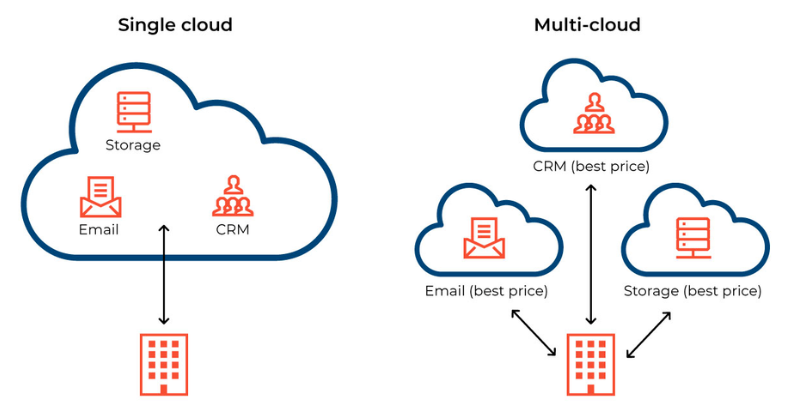
\includegraphics[width=1\textwidth]{images/jpg/multicloud.png} % Ajusta el tamaño seg{\'u}n necesites
                \caption{Simple Cloud y Multicloud}
                \label{fig:SimpleMultiCloud}
            \end{figure}

            El principal objetivo de la arquitectura multinube es incrementar la flexibilidad operativa y evitar la dependencia exclusiva de un solo proveedor (vendor lock-in). A trav{\'e}s de la integraci{\'o}n de dos o m{\'a}s plataformas independientes de nube, las organizaciones pueden desplegar soluciones que mejor se adapten a sus necesidades espec{\'i}ficas, garantizando la disponibilidad y continuidad de los servicios. Este modelo permite utilizar servicios de IaaS (Infraestructura como Servicio), PaaS (Plataforma como Servicio) y SaaS (Software como Servicio) de diferentes proveedores, facilitando una arquitectura robusta y diversificada.
            
            \subsubsection{Ventajas de la Estrategia Multinube}
                Antes de explorar sus beneficios, es importante destacar que la adopci{\'o}n de una estrategia multinube responde a la necesidad de las organizaciones de maximizar el valor de sus inversiones en tecnolog{\'i}a. Esta estrategia se ha convertido en una pr{\'a}ctica com{\'u}n entre empresas que buscan agilidad, escalabilidad y resiliencia en sus operaciones digitales.
                
                Principales ventajas:
                \begin{itemize}
                    \item Reducci{\'o}n del riesgo de dependencia de un {\'u}nico proveedor: Al distribuir las cargas de trabajo entre diferentes plataformas, se minimiza la dependencia de un solo proveedor, lo que otorga mayor libertad y control en la gesti{\'o}n de recursos.
                    \item Optimizaci{\'o}n de costos: La competencia entre proveedores y la posibilidad de seleccionar el servicio que mejor se ajuste a cada necesidad espec{\'i}fica permiten lograr una mejor relaci{\'o}n costo-beneficio.
                    \item Alta disponibilidad y continuidad del negocio: La distribuci{\'o}n de recursos entre diferentes nubes garantiza mayor resiliencia ante ca{\'i}das o fallos en alguna de las plataformas, mejorando la continuidad operativa.
                    \item Flexibilidad y escalabilidad: Se facilita la adopci{\'o}n de nuevas tecnolog{\'i}as y servicios, ampliando la capacidad de respuesta ante cambios en la demanda o en el entorno competitivo.
                    \item Mejora del desempeño: Permite alojar aplicaciones y servicios en ubicaciones geogr{\'a}ficas estrat{\'e}gicas, optimizando la latencia y la experiencia del usuario final.
                \end{itemize}
            \subsubsection{Desaf{\'i}os de la Estrategia Multinube}
                Si bien la arquitectura multinube ofrece m{\'u}ltiples beneficios, tambi{\'e}n implica una serie de retos que las organizaciones deben considerar cuidadosamente antes de su adopci{\'o}n. La complejidad en la gesti{\'o}n y el aseguramiento de la interoperabilidad son algunos de los principales desaf{\'i}os de esta estrategia.

                Principales desaf{\'i}os:
                \begin{itemize}
                    \item Complejidad en la gesti{\'o}n: Administrar m{\'u}ltiples entornos de nube con diferentes pol{\'i}ticas, herramientas y modelos de operaci{\'o}n requiere un esfuerzo adicional y habilidades especializadas.
                    \item Interoperabilidad e integraci{\'o}n: Asegurar que los sistemas y aplicaciones funcionen de manera coherente en plataformas heterog{\'e}neas puede ser complicado, especialmente cuando se manejan diferentes est{\'a}ndares y tecnolog{\'i}as.
                    \item Seguridad y cumplimiento normativo: La diversificaci{\'o}n de proveedores incrementa la dificultad para mantener controles de seguridad consistentes y cumplir con regulaciones espec{\'i}ficas en distintas jurisdicciones.
                    \item Costos ocultos y control financiero: Si no se gestiona adecuadamente, el uso de m{\'u}ltiples proveedores puede generar gastos imprevistos y dificultar el seguimiento preciso de los costos de operaci{\'o}n.
                    \item Gobernanza y control de datos: Es fundamental establecer pol{\'i}ticas claras de gobernanza para evitar problemas de dispersi{\'o}n de datos, accesos no autorizados y garantizar la integridad de la informaci{\'o}n.
                \end{itemize}
}